% Preamble
\documentclass[11pt]{article}

% Packages
\usepackage{amsmath}
\usepackage{amssymb}
\usepackage{wasysym}
\usepackage[makeroom]{cancel}
\usepackage[utf8]{inputenc}
\usepackage[catalan]{babel}
\usepackage{minted}
\usepackage{datetime}
\usepackage{enumerate}
\usepackage{graphicx}
\usemintedstyle{vs}
\setlength{\parindent}{0pt}
% Document
\begin{document}
    \textbf{Arbres binaris equilibrats:
    Quina és la propietat principal o característica dels arbres binaris equilibrats?
    Són equilibrats els següents arbres binaris?
    Raona la teva resposta. }\\

    La propietat principal dels arbres binaris equilibrats és que l'alçada dels seus dos fills difereix, com a molt, en 1.\\

    \textbf{ Arbre binari 1:}\\

    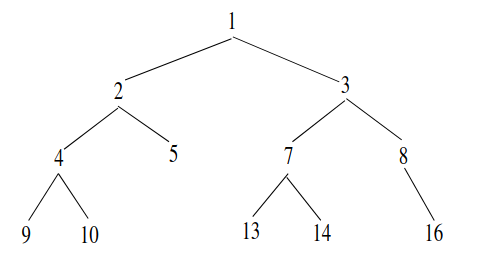
\includegraphics[scale=0.45]{imgs/a1} 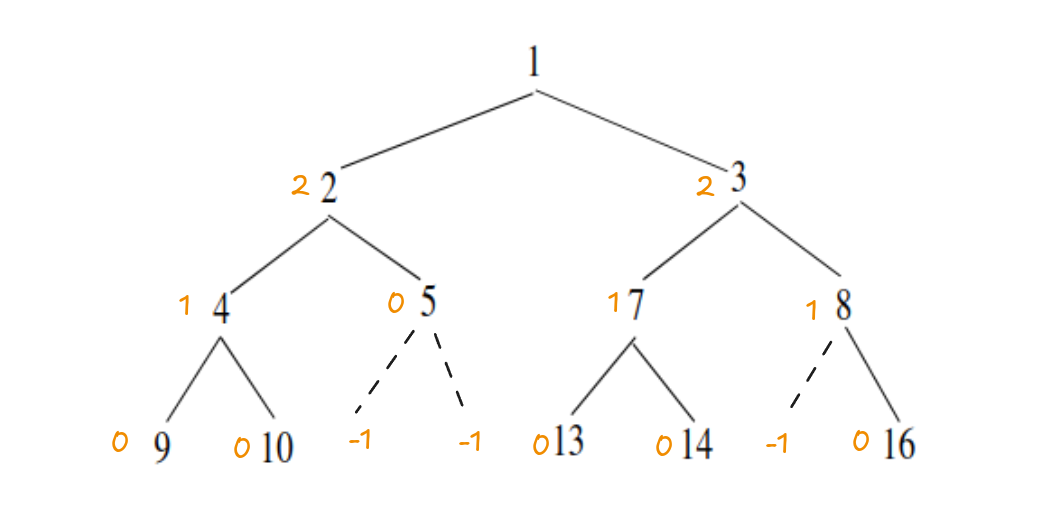
\includegraphics[scale=0.25]{imgs/a1eq}\\

    Com podem veure, no hi ha germans en què l'alçada canviï més d'1, per tant \textbf{SÍ} és equilibrat.\\

    \textbf{ Arbre binari 2:}\\

    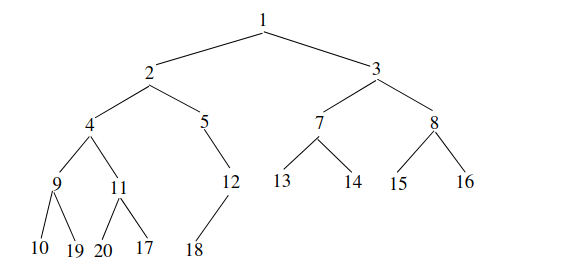
\includegraphics[scale=0.4]{imgs/a2} 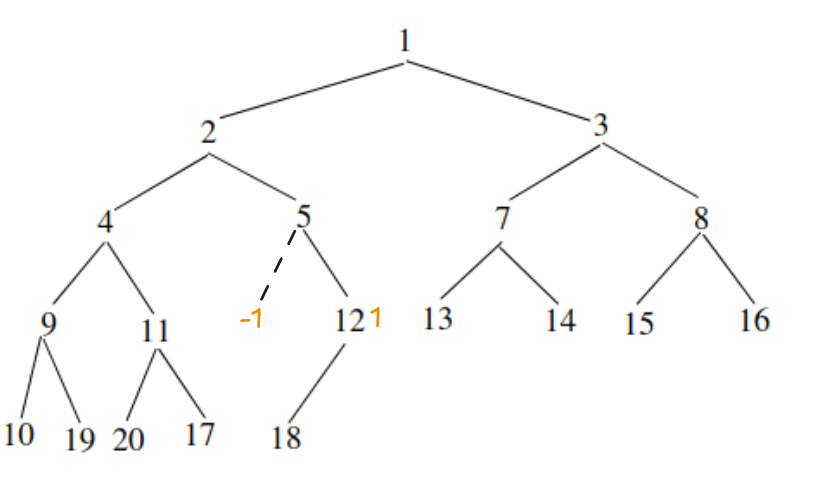
\includegraphics[scale=0.25]{imgs/a2neq}\\

    Com podem veure, ja hem trobat que els dos fills del node 5 tenen altura -1 i 1, i la seva diferència és 2, per tant \textbf{NO} és equilibrat.\\

\end{document}